\newcommand{\UseWhiteBackground}{1}  % Copy this to have a white document
\documentclass[]{scrarticle}
% \newcommand{\lang}{french}  % Copy this in a french document
% \newcommand{\UseWhiteBackground}{1}  % Copy this to have a white document

\usepackage[utf8]{inputenc}
\usepackage{standalone}
\usepackage{etoolbox}
\ifdef{\lang}{}{\newcommand{\lang}{english}}  % If no \lang command is defined, default to english
\usepackage[\lang]{babel}
\usepackage{amssymb,amsmath,amsthm,epsfig,eepic,epic,verbatim,moreverb,fancybox}
\usepackage{stmaryrd}  % for \llbracket and \rrbracket
\usepackage{wasysym}
% \usepackage{bbold}  % NO! DON"T USE IT. It add mathbb for integers but makes it ugly for letters.
\usepackage{dsfont}
% \usepackage{tocstyle}  % To change the table of contents (TOC) style, and that's what we do next
% \usetocstyle{nopagecolumn}  % One of classic, KOMAlike, nopagecolumn, allwithdot, noonewithdot, standard
\usepackage{tikz}
\usepackage{tikz-cd}
\usetikzlibrary{calc,math,decorations.markings,decorations.pathmorphing,arrows,shadows,shapes.geometric,shapes.multipart,patterns,automata,backgrounds}
\usepackage{rotating}  % To have large figures in lanscape with \begin{sidewaysfigure} ... \end{sidewaysfigure}
\usepackage{pdflscape}  % To change one page to landscape
\usepackage{multicol}  % For the \begin{multicol}{N} environement
\usepackage{wrapfig}   % For the \begin{wrapfig}{r|l}{4cm} environement that behave like html float
\usepackage{subcaption}  % To use the subfigure environement in figure environements
\usepackage{multirow}  % Use \multirow{N}{*}{text} to have text in N rows in a table
\usepackage{mathtools}  % For the \xSOMETHINGarrow that we can write on top and change length
\usepackage{xspace}  % To add a space in commands when the following is not pounctuation
\usepackage{todonotes}  % To add todos in the margin of a document with \todo. Also \listoftodos is nice !
\usepackage{graphicx}  % many operations like rotating text etc...
\usepackage{ifthen}
\usepackage{xifthen}
\usepackage{float}  % To have the [H] option for figure so that they don't float. Use only if really needed.
\usepackage{pdfpages}
\usepackage{tablefootnote}  % To have footnotes in tables, use \tablefootnote{...}
\usepackage{enumerate}  % To be able to change the numbering of enumerate environements with [i)] or [a.]...
\usepackage{enumitem}  % To manage the spacing of items and margins
\usepackage{forest}  % For automatic tikz layout
\usepackage[framemethod=tikz]{mdframed}  % Frame around theorems
\usepackage{thmtools}  % Fixes the issue with \autoref and shared counters for thm env. Probably lots of other things also...
\usepackage{listings}
% \usepackage{minted}
\usepackage{pbox}  % A variable width parbox
\usepackage{xcolor}

\definecolor{airforceblue}{rgb}{0.36, 0.54, 0.66}
\definecolor{awesome}{rgb}{1.0, 0.13, 0.32}
\definecolor{bondiblue}{rgb}{0.0, 0.58, 0.71}
\definecolor{atomictangerine}{rgb}{1.0, 0.6, 0.4}
\definecolor{ghostwhite}{rgb}{0.97, 0.97, 1.0}

% creamy background
\ifdef{\UseWhiteBackground}{  % White, default
    \definecolor{myBGcolor}{HTML}{FFFFFF}
    \definecolor{myTextcolor}{HTML}{000000}
    \definecolor{linkColor}{HTML}{044F67}

    % \colorlet{linkColor}{orange!60!blue}
    \colorlet{myRed}{awesome!10!myBGcolor}
    \colorlet{myGreen}{airforceblue!15!myBGcolor}
}{  % Cream
    \definecolor{myBGcolor}{HTML}{E6E0C6}
    \definecolor{myTextcolor}{HTML}{2F251C}
    \colorlet{linkColor}{orange!70!blue}

    \pagecolor{myBGcolor}
    \color{myTextcolor}

    \colorlet{myRed}{awesome!10!myBGcolor}
    \colorlet{myGreen}{green!10!myBGcolor}
}


\usepackage{hyperref}  % Always include it last, as it overrides a lot of commands.
\hypersetup{
    % bookmarks=true,
    % pdfpagemode=FullScreen,  % Only for presentations
    pdfauthor={Diego Dorn},
    pdftitle={ok},
    colorlinks=true,
    allcolors=linkColor
    % linkcolor=blue,
    % urlcolor={winered},
    % filecolor={winered},
    % citecolor={winered},
    % allcolors={orange},
    % linktoc=all,
}

% \usepackage{cleveref}  % Needs to be after hyperref

\addto\extrasenglish{%
    \renewcommand{\subsectionautorefname}{Section}  % Change name of subsection in autoref to be more uniform
}


% Tool to translate commands
% The first argument is the english text, the second is in french
\newcommand{\ifenglish}[2]{\ifthenelse{\equal{\lang}{english}}{#1}{#2}}

% Frames
\mdfdefinestyle{theoremstyle}{%
roundcorner=0pt, % round corners, makes it friendlier
leftmargin=1pt, rightmargin=1pt, % this helps with box warnings
innerbottommargin=12pt,
hidealllines=true, % even friendlier
align=center, %
}

% Theorem environements
\theoremstyle{definition}   % Not in italics
\ifenglish{
    \newtheorem{theorem}{Theorem}[section]
    \newtheorem*{theorem*}{Theorem}
    \newtheorem{theoremx}{Theorem}
    \newtheorem{definition}[theorem]{Definition}
    \newtheorem{notation}[theorem]{Notation}
    \newtheorem{corollary}[theorem]{Corollary}
    \newtheorem{proposition}[theorem]{Proposition}
    \newtheorem*{proposition*}{Proposition}
    \newtheorem{lemma}[theorem]{Lemma}
    \newtheorem*{lemma*}{Lemma}
    \newtheorem*{remark}{Remark}
    \newtheorem*{claim}{Claim}
    \newtheorem*{example}{Example}
    \newtheorem*{examples}{Examples}
    \newtheorem*{exercise}{Exercise}
}{
    \newtheorem{theorem}{Théorème}[section]
    \newtheorem*{theorem*}{Théorème}
    \newtheorem{theoremx}{Théorème}
    \newtheorem{definition}[theorem]{Définition}
    \newtheorem{notation}[theorem]{Notation}
    \newtheorem{corollary}[theorem]{Corrolaire}
    \newtheorem{proposition}[theorem]{Proposition}
    \newtheorem{lemma}[theorem]{Lemme}
    \newtheorem*{remark}{Remarque}
    \newtheorem*{claim}{Assertion}
    \newtheorem*{example}{Exemple}
    \newtheorem*{examples}{Exemples}
    \newtheorem*{exercise}{Exercise}
}
\renewcommand{\thetheoremx}{\Alph{thmx}} % "letter-numbered" theorems


\surroundwithmdframed[style=theoremstyle,backgroundcolor=myRed]{theorem}
\surroundwithmdframed[style=theoremstyle,backgroundcolor=myRed]{theorem*}
\surroundwithmdframed[style=theoremstyle,backgroundcolor=myGreen]{definition}

%%%%%%%%%%%%%%%%%%%
%   Parenthesis   %
%%%%%%%%%%%%%%%%%%%

\newcommand{\parenthesis}[1]{\left(#1\right)}
\newcommand{\bigparenthesis}[1]{\big(#1\big)}
\newcommand{\Bigparenthesis}[1]{\Big(#1\Big)}
\newcommand{\Par}[2][]{
    \ifthenelse{\isempty{#1}}{%
        \mathopen{}\left(#2\right)\mathclose{}%
    }{\ifthenelse{#1 = 0}{
        (#2)%
    }{\ifthenelse{#1 = 1}{%
        \big(#2\big)%
    }{\ifthenelse{#1 = 2}{%
        \Big(#2\Big)%
    }{\ifthenelse{#1 = 3}{%
        \large(#2\large)%
    }{\ifthenelse{#1 = 4}{%
        \Large(#2\Large)%
    }{%
        \mathopen{}\left(#2\right)\mathclose{}%
    }}}}}}}
\newcommand{\Bra}[2][]{
    \ifthenelse{\isempty{#1}}{%
        \mathopen{}\left[#2\right]\mathclose{}%
    }{\ifthenelse{#1 = 0}{
        [#2]%
    }{\ifthenelse{#1 = 1}{%
        \big[#2\big]%
    }{\ifthenelse{#1 = 2}{%
        \Big[#2\Big]%
    }{\ifthenelse{#1 = 3}{%
        \large[#2\large]%
    }{\ifthenelse{#1 = 4}{%
        \Large[#2\Large]%
    }{%
        \mathopen{}\left[#2\right]\mathclose{}%
    }}}}}}}


\newcommand{\brackets}[1]{\left[#1\right]}

%%%%%%%%%%%%%%%%%%%
%    Operators    %
%%%%%%%%%%%%%%%%%%%

\DeclareMathOperator{\id}{id}
\DeclareMathOperator{\re}{Re}
\DeclareMathOperator{\Aut}{Aut}
\DeclareMathOperator{\Hom}{Hom}
\DeclareMathOperator{\Char}{char}
\DeclareMathOperator{\im}{Im}
\DeclareMathOperator{\dom}{dom}
\DeclareMathOperator{\cof}{cof}
\DeclareMathOperator{\Ob}{Ob}
\DeclareMathOperator{\Mor}{Mor}
\DeclareMathOperator{\rk}{rk}

\newcommand{\concat}{
  \mathord{
    \mathchoice
    {\raisebox{1ex}{\scalebox{.7}{$\frown$}}}
    {\raisebox{1ex}{\scalebox{.7}{$\frown$}}}
    {\raisebox{.7ex}{\scalebox{.5}{$\frown$}}}
    {\raisebox{.7ex}{\scalebox{.5}{$\frown$}}}
  }
}
\newcommand{\restr}[1]{\mathbin\upharpoonright_{#1}}
\newcommand{\compl}[1]{#1^\mathsf{c}}
\newcommand{\abs}[1]{\left| #1 \right|}
\newcommand{\bigabs}[1]{\big\lvert#1\big\rvert}
\newcommand{\parens}[1]{\left(#1\right)}
\newcommand{\norm}[1]{\left\| #1 \right\|}

%%%%%%%%%%%%%%%%%%%
%  Constructions  %
%%%%%%%%%%%%%%%%%%%

% Arrows
\newcommand{\xto}[1]{\xrightarrow{#1}}

% Structures
\newcommand{\verteqsign}{\rotatebox{90}{$\,=$}}
\newcommand{\verteq}[2]{\underset{\scriptstyle\overset{\mkern4mu\verteqsign}{#2}}{#1}}
\newcommand{\vertimplies}[2]{\underset{\scriptstyle\overset{\uparrow}{#2}}{#1}}
\newcommand{\func}[5]{
    \begin{array}{rccl}
            #1 : & #2 & \longrightarrow & #3 \\
                 & #4 & \longmapsto     & #5
    \end{array}
}
\newcommand{\ntimes}[2]{\underbrace{#1, \dots, #1}_{#2 \ttimes}}
% Reminder: for combinations / binomial coefficients, use \binom{n}{k}

% Set definitions
\newcommand{\set}[1]{\left\{ #1 \right\}}
\newcommand{\bigset}[1]{\big\{ #1 \big\}}
\newcommand{\setst}[2]{\left\{ #1 \, \middle| \, #2 \right\}}
\newcommand{\bigsetst}[2]{\big\{ #1 \, \big| \, #2 \big\}}

\newcommand{\funcset}[2]{{}^{#1}{#2}}
\newcommand{\angles}[1]{\left\langle #1 \right\rangle}
\newcommand{\brz}{B_r(z_0)}
\newcommand\quotient[2]{
    \mathchoice
        {% \displaystyle
            \text{\raise1ex\hbox{$#1$}\Big/\lower1ex\hbox{$#2$}}%
        }
        {% \textstyle
            #1\,/\,#2
        }
        {% \scriptstyle
            #1\,/\,#2
        }
        {% \scriptscriptstyle
            #1\,/\,#2
        }
}
\newcommand{\interior}[1]{\mathring{#1}}

%%%%%%%%%%%%%%%
%   Letters   %
%%%%%%%%%%%%%%%


% Greek alphabe
\renewcommand{\phi}{\ensuremath\varphi\xspace}
\renewcommand{\epsilon}{\ensuremath\varepsilon\xspace}
\renewcommand{\a}{\ensuremath\alpha\xspace}
\renewcommand{\d}{\ensuremath{\partial}\xspace}
\newcommand{\D}{\ensuremath\Delta\xspace}
\newcommand{\e}{\ensuremath\epsilon\xspace}
\newcommand{\g}{\ensuremath\gamma\xspace}
\newcommand{\y}{\g}  % I mistake them every other time
\newcommand{\p}{\phi\xspace}
\newcommand{\s}{\sigma\xspace}
\newcommand{\w}{\ensuremath\omega\xspace}

% Mathbb alphabet

\newcommand{\IB}{\ensuremath{\mathbb B}\xspace}
\newcommand{\C}{\ensuremath{\mathbb C}\xspace}
\newcommand{\ID}{\ensuremath{\mathbb D}\xspace}
\newcommand{\IE}{\ensuremath{\mathbb E}\xspace}
\newcommand{\F}{\ensuremath{\mathbb F}\xspace}
\newcommand{\IG}{\ensuremath{\mathbb G}\xspace}
\newcommand{\N}{\ensuremath{\mathbb N}\xspace}
\newcommand{\R}{\ensuremath{\mathbb R}\xspace}
\newcommand{\IP}{\ensuremath{\mathbb P}\xspace}
\newcommand{\IS}{\ensuremath{\mathbb S}\xspace}
\newcommand{\IT}{\ensuremath{\mathbb T}\xspace}
\newcommand{\Q}{\ensuremath{\mathbb Q}\xspace}
\newcommand{\Z}{\ensuremath{\mathbb Z}\xspace}
\newcommand{\ONE}{\text{\usefont{U}{bbold}{m}{n}1}}

% Fancy fonts
\newcommand{\Aa}{\ensuremath{\mathcal A}\xspace}
\newcommand{\Bb}{\ensuremath{\mathcal B}\xspace}
\newcommand{\Cc}{\ensuremath{\mathcal C}\xspace}
\newcommand{\Dd}{\ensuremath{\mathcal D}\xspace}
\newcommand{\Ee}{\ensuremath{\mathcal E}\xspace}
\newcommand{\Ff}{\ensuremath{\mathcal F}\xspace}
\newcommand{\Gg}{\ensuremath{\mathcal G}\xspace}
\newcommand{\Hh}{\ensuremath{\mathcal H}\xspace}
\newcommand{\Ii}{\ensuremath{\mathcal I}\xspace}
\newcommand{\Jj}{\ensuremath{\mathcal J}\xspace}
\newcommand{\Kk}{\ensuremath{\mathcal K}\xspace}
\newcommand{\Ll}{\ensuremath{\mathcal L}\xspace}
\newcommand{\Mm}{\ensuremath{\mathcal M}\xspace}
\newcommand{\Nn}{\ensuremath{\mathcal N}\xspace}
\newcommand{\Oo}{\ensuremath{\mathcal O}\xspace}
\newcommand{\Pp}{\ensuremath{\mathcal P}\xspace}
\newcommand{\Qq}{\ensuremath{\mathcal Q}\xspace}
\newcommand{\Rr}{\ensuremath{\mathcal R}\xspace}
\newcommand{\Ss}{\ensuremath{\mathcal S}\xspace}
\newcommand{\Tt}{\ensuremath{\mathcal T}\xspace}
\newcommand{\Uu}{\ensuremath{\mathcal U}\xspace}
\newcommand{\Vv}{\ensuremath{\mathcal V}\xspace}
\newcommand{\Ww}{\ensuremath{\mathcal W}\xspace}
\newcommand{\Xx}{\ensuremath{\mathcal X}\xspace}
\newcommand{\Yy}{\ensuremath{\mathcal Y}\xspace}
\newcommand{\Zz}{\ensuremath{\mathcal Z}\xspace}
\renewcommand{\O}[1]{\mathcal{O}\left(#1\right)}

% Others
\renewcommand{\emptyset}{\varnothing}


%%%%%%%%%%%%%%%%%%
%   New symbols  %
%%%%%%%%%%%%%%%%%%

\newcommand{\iddots}{{\cdot^{\cdot^\cdot}}}  % Three dots on the antidiagonal
\newcommand{\existsinf}{\exists^\infty}
\newcommand{\coloneq}{\mathrel{\resizebox{\widthof{$\mathord{=}$}}{\height}{ $\!\!\resizebox{1.2\width}{0.8\height}{\raisebox{0.23ex}{$\mathop{:}$}}\!\!=\!\!$ }}}  % Fancier :=

%%%%%%%%%%%%%%%%%%
%   Shorthands   %
%%%%%%%%%%%%%%%%%%

% Math text
\newcommand{\open}{\text{ open }}
\newcommand{\st}{\text{ \ifenglish{s.t}{t.q}. }}
\newcommand{\andd}{\text{ \ifenglish{and}{et} }}
\newcommand{\andquad}{\quad\andd\quad}
\newcommand{\et}{\text{ et }}
\newcommand{\ttimes}{\text{ times}}
\newcommand{\tif}{\text{if }}
\newcommand{\otherwise}{\text{otherwise}}

% Symbols
\newcommand{\acts}{\circlearrowright}
\newcommand{\sub}{\subset}
\newcommand{\subeq}{\subseteq}
\renewcommand{\iff}{\ensuremath{\Longleftrightarrow}}
\newcommand{\iffquad}{\quad\iff\quad}
\newcommand{\del}{\partial}
\newcommand{\x}{\times}
\renewcommand{\emph}{\textbf}
\newcommand{\Forces}{\vdash}

%%%%%%%%%%%%%%%%%%%%
% Subject specific %
%%%%%%%%%%%%%%%%%%%%

% Maybe those should go inside their respesective files

% Graph theory
\DeclareMathOperator*{\ex}{ex}
\newcommand{\Turan}{\mathcal{T}}

% Analytic number theory
\newcommand{\sumdn}{\sum_{d|n}}
\newcommand{\Li}{\mathrm{Li}}

% Smooth manifolds
\newcommand{\chart}[1]{(\phi_{#1}, U_{#1})}
\newcommand{\der}[1]{\frac{\del}{\del #1}}

% Galois Theory
\newcommand{\clot}[1]{\overline{#1}}
\newcommand{\Gal}{\mathrm{Gal}}
% \DeclareMathOperator*{\Gal}{Gal}
\newcommand{\Kxx}{K[x_1, \dots, x_n]}

% Algebraic topology
\newcommand{\HCW}{H^{\mathrm{CW}}}

% Complexity
\newcommand{\coP}{\mathsf{coP}}
\newcommand{\Ptime}{\mathsf{P}}
\newcommand{\PHierachy}{\mathsf{PH}}
\newcommand{\NP}{\mathsf{NP}}
\newcommand{\coNP}{\mathsf{coNP}}
\newcommand{\PSPACE}{\mathsf{PSPACE}}
\newcommand{\NPSPACE}{\mathsf{NPSPACE}}

% Analysis
\newcommand{\dd}{\mathrm{d}}

% Probability

% Neural networks
\newcommand{\MSE}{\mathrm{MSE}}
\newcommand{\KLdiv}[3][]{D_{\mathrm{KL}}\Par[#1]{#2 \mid\mid #3}}
\DeclareMathOperator{\Sign}{Sign}
% A Devil emoji in exponent of the argument
\newcommand{\Adversarial}[1]{#1^{\raisebox{-0.2ex}{
\includegraphics[height=2ex]{images/devil.png}}}}

% Logic
\newcommand{\Symbol}[1]{\underline{#1}}

% Descriptive Set Theory
\newcommand{\baire}{\ensuremath{\w^\w}\xspace}
\newcommand{\cantor}{\ensuremath{2^\w}\xspace}
\newcommand{\W}{\ensuremath{\w_1}\xspace}  % This is meant to be used only for the first uncountable ordinal
% Classes
\newcommand{\bS}[1]{\ensuremath{\mathbf{\Sigma}^0_{#1}}\xspace}
\newcommand{\bP}[1]{\ensuremath{\mathbf{\Pi}^0_{#1}}\xspace}
\newcommand{\bD}[1]{\ensuremath{\mathbf{\Delta}^0_{#1}}\xspace}
\newcommand{\borelsigma}[1]{\ensuremath{\mathbf{\Sigma}^0_{#1}}\xspace}
\newcommand{\borelpi}[1]{\ensuremath{\mathbf{\Pi}^0_{#1}}\xspace}
\newcommand{\boreldelta}[1]{\ensuremath{\mathbf{\Delta}^0_{#1}}\xspace}
\newcommand{\borelGamma}{\ensuremath{\mathbf{\Gamma}}\xspace}
\newcommand{\LambdaClass}[2]{\ensuremath{\mathbf{\Lambda}_{#1, #2}}\xspace}
\newcommand{\dualclass}[1]{\check{#1}}
\newcommand{\nsd}{non-self-dual\xspace}
\newcommand{\projectivesigma}[1]{\ensuremath{\mathbf{\Sigma}^1_{#1}}\xspace}
\newcommand{\projectivepi}[1]{\ensuremath{\mathbf{\Pi}^1_{#1}}\xspace}
\newcommand{\projectivedelta}[1]{\ensuremath{\mathbf{\Delta}^1_{#1}}\xspace}
% Sets of sequences
\newcommand{\seqlt}[2]{{#2}^{<#1}}
\newcommand{\finiteseq}[1]{\seqlt{\w}{#1}}
% \newcommand{\infseq}[1]{\funcset{\omega}{#1}}
% \newcommand{\allseq}[1]{\funcset{\leq\omega}{#1}}
\newcommand{\infseq}[1]{{#1}^\w}
\newcommand{\allseq}[1]{{#1}^{\leq\omega}}
\newcommand{\finitebaire}{\ensuremath{\finiteseq{\w}}\xspace}
\newcommand{\finitecantor}{\ensuremath{\finiteseq{2}}\xspace}
\newcommand{\length}[1]{\mathrm{lh}(#1)}
\newcommand{\emptyseq}{\langle\rangle}
% Operators
\renewcommand{\succ}[2][]{\ifthenelse{\isempty{#1}}{\mathrm{succ}(#2)}{\mathrm{succ}_{#1}(#2)}}
\DeclareMathOperator{\odd}{odd}
\DeclareMathOperator{\even}{even}
\DeclareMathOperator{\last}{last}
\newcommand{\Countf}[1]{\#_{#1}}
\newcommand{\difference}[1]{D_{#1}}
\newcommand{\suffixes}[2]{{#1}_{(#2)}}
\newcommand{\wadd}{\oplus}
\newcommand{\wCountableSup}{\mathrm{sup^\w}}
\newcommand{\wmult}{\mathop{\otimes}}
\newcommand{\bigeraser}{\ensuremath{\mathord{\Uparrow}}\xspace}
\renewcommand{\interleave}{\mathbin{\S}}
\newcommand{\Init}[1]{\mathrm{Init}_{#1}}
% Players
\newcommand{\I}{\texttt{I}\xspace}
\newcommand{\II}{\texttt{II}\xspace}
\newcommand{\playerA}{Player \I}
\newcommand{\playerB}{Player \II}

% \renewcommand{\I}{\texttt{M}\xspace}
% \renewcommand{\II}{\texttt{B}\xspace}
% \renewcommand{\playerA}{Michael\xspace}
% \renewcommand{\playerB}{Bob\xspace}
% Wadge
\newcommand{\leW}{\le_\textsc{w}}
\newcommand{\geW}{\ge_\textsc{w}}
\newcommand{\gtW}{>_\textsc{w}}
\newcommand{\ltW}{<_\textsc{w}}
\newcommand{\equivW}{\equiv_\textsc{w}}
\newcommand{\Wdegree}[1]{[#1]_{\equivW}}
% Axioms / Theories
\newcommand{\ZF}{\textbf{ZF}\xspace}
\newcommand{\ZFC}{\textbf{ZFC}\xspace}
\newcommand{\AD}{\textbf{AD}\xspace}
\renewcommand{\AC}{\textbf{AC}\xspace}
\newcommand{\DC}{\textbf{DC}\xspace}
% Games
\newcommand{\GaleStewart}[1]{\ensuremath{G(#1)}\xspace}
\newcommand{\BanachMazur}[1]{\ensuremath{BM(#1)}\xspace}
\newcommand{\Wadge}[2]{\ensuremath{G(#1, #2)}\xspace}
% Automatons
\newcommand{\automaton}{automatic set\xspace}
\newcommand{\automata}{automatic sets\xspace}
\newcommand{\Automata}{Automatic sets\xspace}
\newcommand{\Language}{\mathcal{L}}
\DeclareMathOperator{\Inf}{Inf}
\newcommand{\AcceptanceCondition}{\mathrm{Acc}}
\newcommand{\automatonMinus}{\scalebox{0.5}{\begin{tikzpicture}[automata, baseline=-2mm]
    \node[minus] {};
\end{tikzpicture}}\xspace}
\newcommand{\automatonPlus}{\scalebox{0.5}{\begin{tikzpicture}[automata, baseline=-2mm]
    \node[plus] {};
\end{tikzpicture}}\xspace}
\newcommand{\automatonState}[1]{\scalebox{0.5}{\begin{tikzpicture}[automata, baseline=-2mm, minimum size=20]
    \node[state] {\Large \(#1\)};
\end{tikzpicture}}\xspace}
\newcommand{\sumAutomaton}[2]{\begin{tikzpicture}[automata]
    \path node[initial, state] (root) {$#2$}
        +(2, 1) node[state] (A) {$#1$}
        +(2, -1) node[state] (Ac) {$\compl{#1}$};
    \draw (root) edge (A) edge (Ac);
\end{tikzpicture}}


%%%%%%%%%%%%%%%%%
%     Tikz      %
%%%%%%%%%%%%%%%%%

\tikzcdset{row sep/normal=1cm, column sep/normal=1cm}  % So tikz-cd diagram are more squared

% Draws irregular circles.
\newcommand{\irregularcircle}[2]{  % radius, irregularity
  let \n1 = {(#1)+rand*(#2)} in
  +(0:\n1)
  \foreach \a in {10,20,...,350}{
    let \n1 = {(#1)+rand*(#2)} in
    -- +(\a:\n1)
  } -- cycle
}

\tikzset{
triangle/.style={ % To create triangles in trees
  draw=myRed!90!black,
  text=black,
  fill=myRed,
  shape border uses incircle,
  isosceles triangle,
  shape border rotate=90,
}}

% Used to make arrows on paths. Use like this: \draw[marr=\Singlearrow]
\tikzset{marr/.style={
  decoration={
    markings,
    mark=at position 0.5 with {#1}
    },
  postaction={decorate}
}}
\def\Singlearrow{{\arrow[scale=1.5,xshift={0.5pt+2.25\pgflinewidth}]{>}}}
\def\Doublearrow{{\arrow[scale=1.5,xshift=1.35pt +2.47\pgflinewidth]{>>}}}
\def\Triplearrow{{\arrow[scale=1.5,xshift=1.75pt +2.47\pgflinewidth]{>>>}}}
\newcommand{\CWarrow}[3]{ [->] ($1/3*(#1) + 1/3*(#2) + 1/3*(#3)$) ++(220:4pt) arc (220:-40:4pt)}
\newcommand{\CCWarrow}[3]{ [->] ($1/3*(#1) + 1/3*(#2) + 1/3*(#3)$) ++(-40:4pt) arc (-40:220:4pt)}

% For automatons
\tikzset{
    initial text={},
    do path picture/.style={%
        path picture={%
        \pgfpointdiff{\pgfpointanchor{path picture bounding box}{south west}}%
            {\pgfpointanchor{path picture bounding box}{north east}}%
        \pgfgetlastxy\x\y%
        \tikzset{x=\x/2,y=\y/2}%
        #1
        }
    },
    automata/.style={
        node distance=60pt,
        minimum size=20,
        every edge/.style={
            draw,
            ->,
            auto,
        }
    },
    plus/.style={
        draw,
        circle,
        do path picture={
            \draw [line cap=round, very thick] (-1/2,0) -- (1/2,0) (0,-1/2) -- (0,1/2);
        }
    },
    minus/.style={
        draw,
        circle,
        do path picture={
            \draw [line cap=round, very thick] (-1/2,0) -- (1/2,0);
        }
    },
    % Removes extra space on initial nodes
    % From: https://tex.stackexchange.com/questions/111554/how-to-avoid-superfluous-space-in-the-initial-state-of-a-tikz-automaton#comment245757_111558
    every initial by arrow/.append style={anchor/.append style={shape=coordinate}},
    state/.append style={fill=white},
}

% To put at the bottom right corner of a square that commutes.
\newcommand{\commutes}{\arrow[ul, phantom, "\scalebox{1.5}{$\circlearrowleft$}"]}

% To link two lines in a long exact sequence.
% First argument is where the line should connect (ex: dll)
% Second argument is the label on the line.
\newcommand{\connecting}[2]{
    \arrow[#1,phantom, ""{coordinate, name=Z}]
    \arrow[#1, "#2", rounded corners,
        to path={
            -- ([xshift=2ex]\tikztostart.east)
            |- (Z)[near start]\tikztonodes
            -| ([xshift=-2ex]\tikztotarget.west)
            -- (\tikztotarget)
        }]
}
\newcommand{\dotsto}{\mathllap{\cdots\longrightarrow\ }}  % ... → indicate the start of a long sequence without taking space
\newcommand{\todots}{\mathrlap{\ \longrightarrow\cdots}}  % → ... indicate the end of a long sequence without taking space

\newenvironment{longsequence}{
    \begin{center}
        \begin{tikzcd}[row sep=0.5cm]
}{
        \end{tikzcd}
    \end{center}
}


\newcommand{\quickfig}[2]{
    \begin{wrapfigure}{r}{40mm}
        \begin{center}
            #2
        \end{center}
        \caption{#1}
    \end{wrapfigure}
}


\title{Between decideable logics: $\mathbf{\omega}$-automata and infinite games}
\author{Diego Dorn}

% \renewcommand{\todo}[1]{}

\begin{document}

\begin{titlepage}
\begin{center}
    \Large
    \textsf{Semester Project -- Autumn 2023}

    \vspace{1em}

    \textbf{\textsf{
        \Huge
        Adversarial Attacks on Autoencoders
    }}

    \begin{center}
        With \total{figure} figures
    \end{center}


    \vfill

    \begin{center}
        \normalsize
        \scalebox{1.0}{
        % \input{fig/muller-1-no-11.tex}
        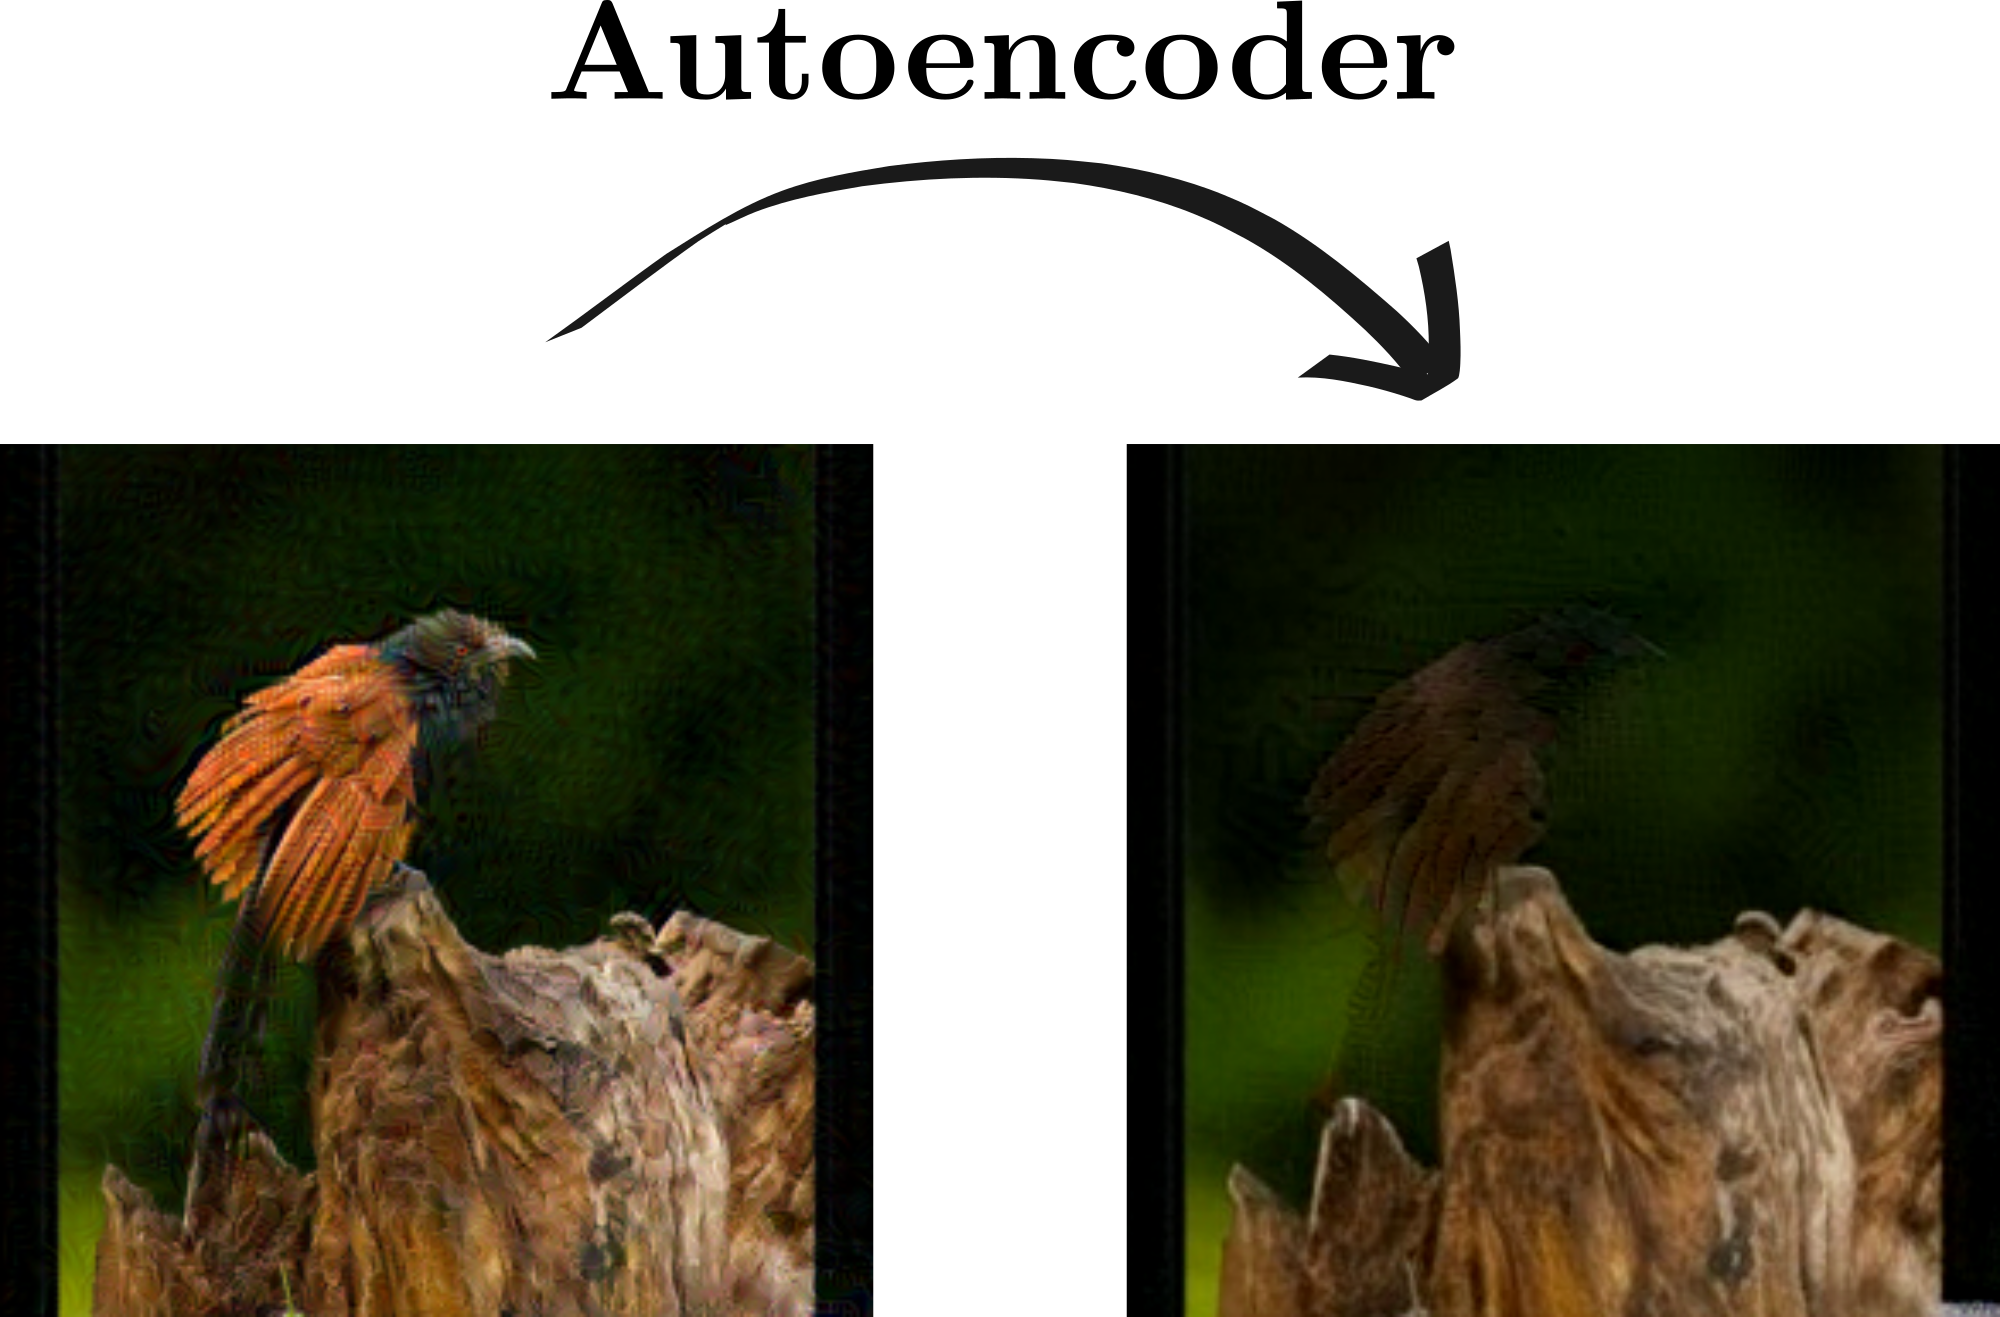
\includegraphics[width=0.8\linewidth]{../images/bird-no-bird.png}
        }
    \end{center}

    \vfill


    \begin{minipage}{0.3\textwidth}
        \textit{Author} \\
        Diego \textsc{Dorn}
    \end{minipage}
    ~
    
\includegraphics[width=3cm]{epfl.png}
    ~
    \begin{minipage}{0.3\textwidth}
        \begin{flushright}
            \textit{Supervisor} \\
            Clément \textsc{Hongler}
        \end{flushright}
    \end{minipage}
    \vspace{1cm}

    \vspace*{-3cm}
\end{center}
\end{titlepage}

\listoftodos[Remaining to be done]
\newpage


% \setcounter{section}{-1}
\section*{Introduction}
\addcontentsline{toc}{section}{Introduction}

Artificial neural networks are famously vulnerable to adversarial attacks
\cite{szegedy2013intriguing,goodfellow2014explaining,liu2021survey}.
\todo{Check the papers}

- defense, autoencoders

- universal, transferable attacks


\tableofcontents

\clearpage
\section*{Conventions}
\addcontentsline{toc}{section}{Conventions}

Throughout this document we adopt a set of conventions and notations.
\begin{itemize}
  \item We use $A \subset B$ to say $A$ is included, not strictly in $B$
    and $A \subsetneq B$ if this inclusion is strict.
  \item $\Xx \subset \R^n$ is the set in which datapoints live.
  \item $\Yy$ is a space of labels, which will most of the time be categorical,
    i.e. $\Yy = \set{0, 1}$ or $\Yy = \set{\text{cat}, \text{dog}, \text{boat}}$.
  \item We use $\Dd$ for datasets. For unlabelled datasets, $\Dd \subset \Xx$.
    For labelled datasets, $\Dd \subset \Xx \times \Yy$.
  \item Loss functions are denoted by $\Ll$.
  \item We write $\norm{\cdot}$ for the euclidean norm on $\R^n$,
    and $\norm{\cdot}_p$ for the $p$-norm on $\R^n$.
    As a reminder, for $x \in \R^n$, $\norm{x}_\infty = \max_{i=1}^n \abs{x_i}$.
\end{itemize}


\clearpage

\section{Attacking classifiers}
The common knowledge is that neural networks are vulnerable to adversarial attacks
and adversarial attacks are easy to find \cite{szegedy2013intriguing,goodfellow2014explaining,liu2021survey}.
The first thing I wanted to do was to verify this in practice. Can I easily
attack any classifier outside of the well defined confines of a classroom
or a paper for which a lot of work was put into?
\todo{Add motivation for why I choose this (philo, impact)}

\subsection{Setup}
I used three different models and datasets throughout this project.
The code of every experiment is available at \url{
  https://github.com/ddorn/autoencoder-attacks
}.

\paragraph{MNIST}
The smallest dataset I used is the MNIST dataset \cite{LeCun1998GradientbasedLA},
with a small convolutional classifier acheiving $98.8\,\%$ accuracy implemented in pytorch \cite{tuomaso2022trainmnistfast}.0

\paragraph{CIFAR-10}
The second dataset is the CIFAR-10 dataset \cite{Krizhevsky2009LearningML},
with a convolutional classifier acheiving $92.8 \%$ accuracy \cite{999912022cifar10fastsimple}.

\begin{figure}[h]
  \centering
  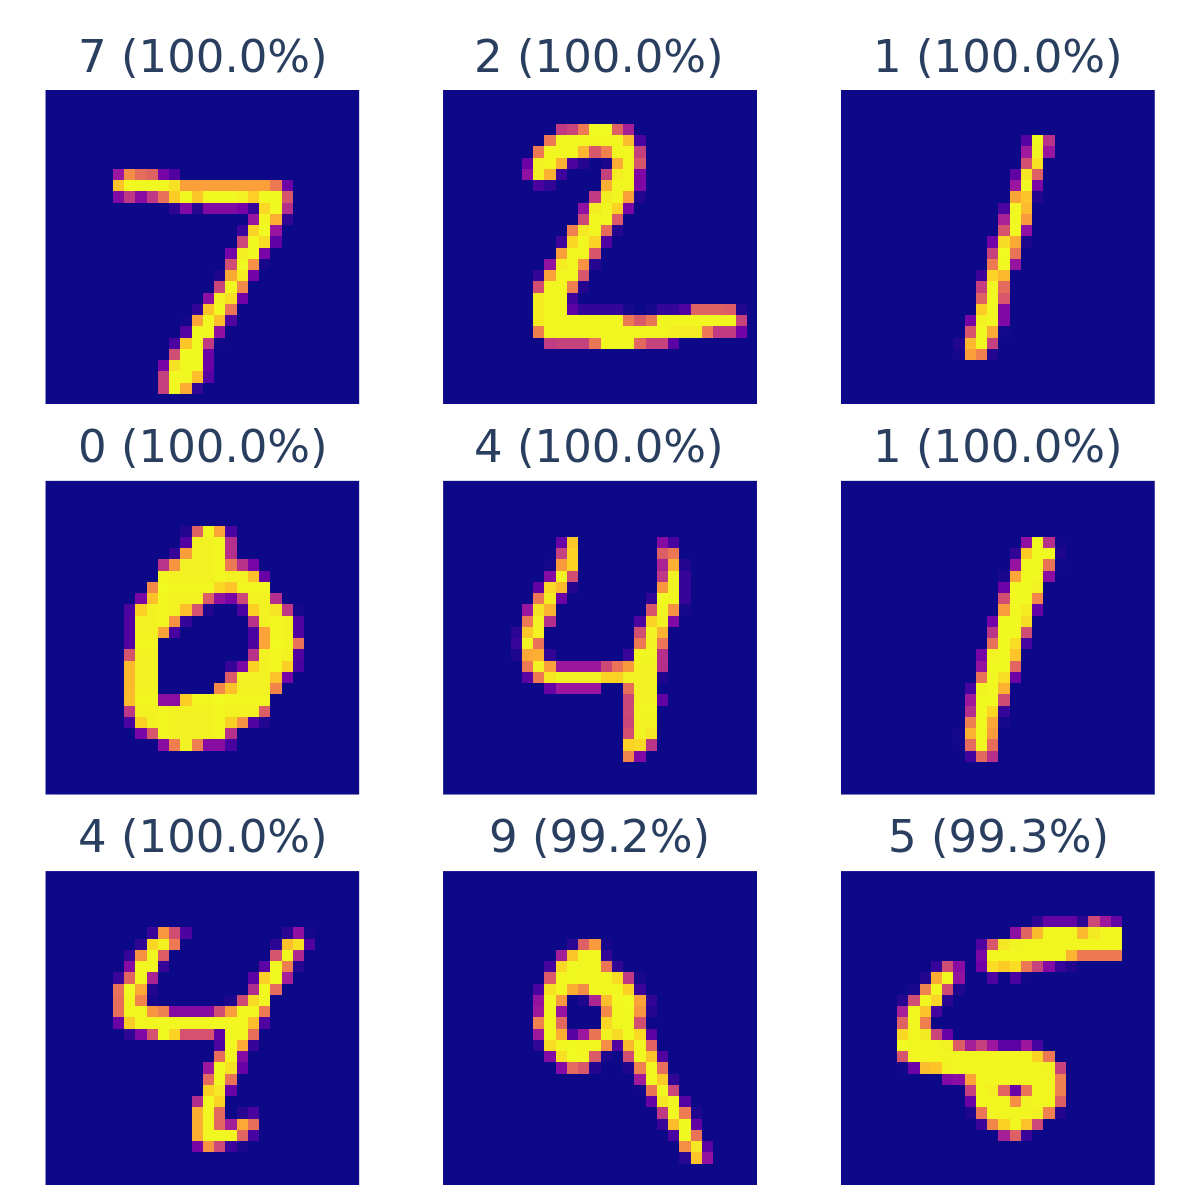
\includegraphics[width=0.45\textwidth]{images/sample_MNIST.png}
  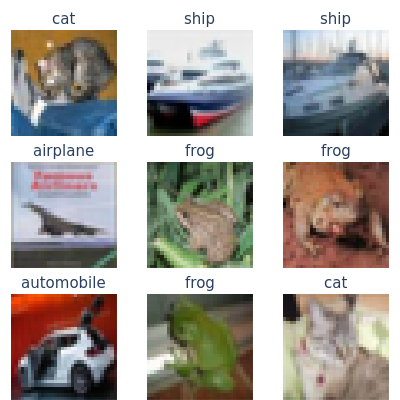
\includegraphics[width=0.45\textwidth]{images/sample_CIFAR10.png}
  \caption{
    The first 9 test images of
    the MNIST dataset (left)
    the CIFAR-10 dataset (right).
    The confidence of the classifier is shown in parenthesis.}
  \label{fig:mnist_cifar10_samples}
\end{figure}


\paragraph{ImageNet}
The third dataset is ImageNet \cite{Deng2009ImageNetAL}, with a ResNet-50 classifier
achieving $77\,\%$ top-1 accuracy \cite{He2015DeepRL}.

\begin{figure}[h]
  \centering
  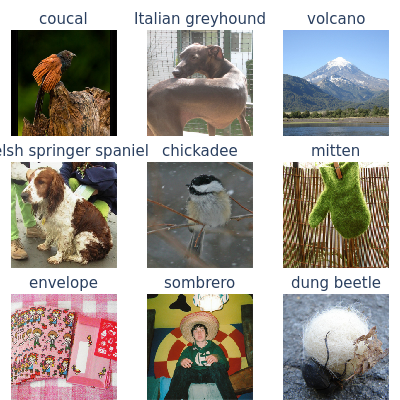
\includegraphics[width=0.45\textwidth]{images/sample_ImageNet.png}
  \caption{The first 9 test images of the ImageNet dataset.
    The confidence of the classifier is shown in parenthesis.}
  \label{fig:imagenet_samples}
\end{figure}


\subsection{Fast gradient sign method}
The simplest attack is the fast gradient sign method (FGSM) \cite{goodfellow2014explaining}.
This attack requires only one forward and one backward pass through the network
to find a small perturbation of an image that can (potentially) fool the classifier.

What is small? We usually constrain the norm of the perturbation to
a small value $\epsilon$. The norm used can be the $l_\infty$ norm,
for $\epsilon = 10 / 255$ or $\epsilon = 4 / 255$ are common values,
or the $l_0$, $l_1$ or $l_2$ norm.
Clearly the four norms produce different constrains, and should be chosen
depending on the context:
\begin{itemize}
  \item $l_\infty$ is a natural choice, and corresponds to changing each
    pixel value by at most $\epsilon$.
    % If $\epsilon \leq 4 / 255$, the perturbation is not visible to the human eye.
  \item Using the $l_0$ norm means to change at most $\epsilon$ pixels. This
    can be one-pixel attacks \cite{Su2017OnePA},
    attacks that change a small number of pixels,
    or patch attacks \cite{Brown2017AdversarialP}.
  \item $l_1$ and $l_2$ constraints can be used when it is fine if
    some pixels are completely changed, but not too many are changed
    a lot.
\end{itemize}

The fast gradient sign method is an untargeted attack, meaning that
the goal is to find a perturbation that changes the prediction of the classifier,
but not to force the classifier to predict a specific label.
It is defined as follows.

\begin{definition}
  Let $f$ be a classifier and $x \in \Xx$ an input.
  The \emph{fast gradient sign method} is the attack that computes
  \[
    %\Adversarial{x}
    x_{\text{FGSM}}
      = x + \epsilon \cdot \Sign \Par{\nabla_x \Ll(f(x), y)}
  \]
  where $\Ll$ is the loss function used to train $f$,
  and $\epsilon$ is the desired $l_\infty$ norm of the perturbation.
\end{definition}

We show an example of the attack on the first test image for each of the
datasets, with the top 5 categories shown in
\autoref{fig:fgsm_examples_mnist}, \autoref{fig:fgsm_examples_cifar10}
and \autoref{fig:fgsm_examples_imagenet}.

% A full page for the figure below, without page numbers
\begin{figure}[H]
  \centering
  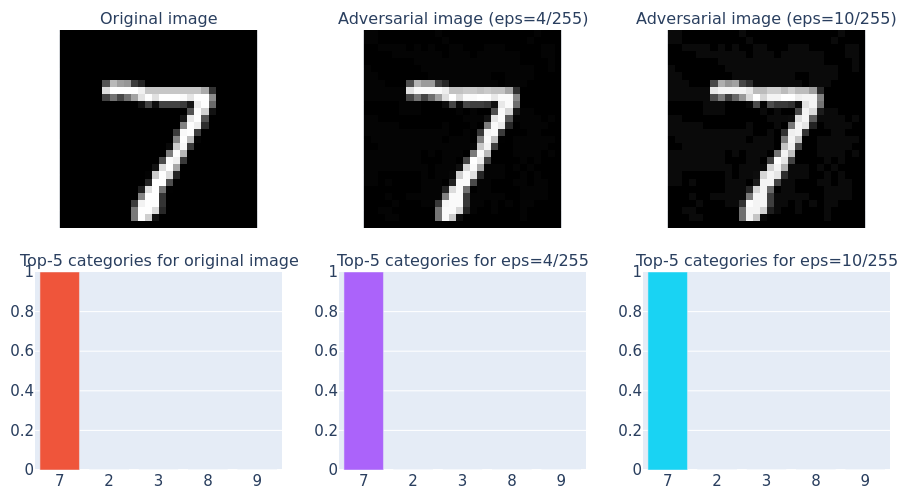
\includegraphics[width=0.9\textwidth]{images/fgsm_example_MNIST.png}
  \caption{Examples of the FGSM attack.}
  \label{fig:fgsm_examples_mnist}
\end{figure}

\begin{figure}[H]
  \centering
  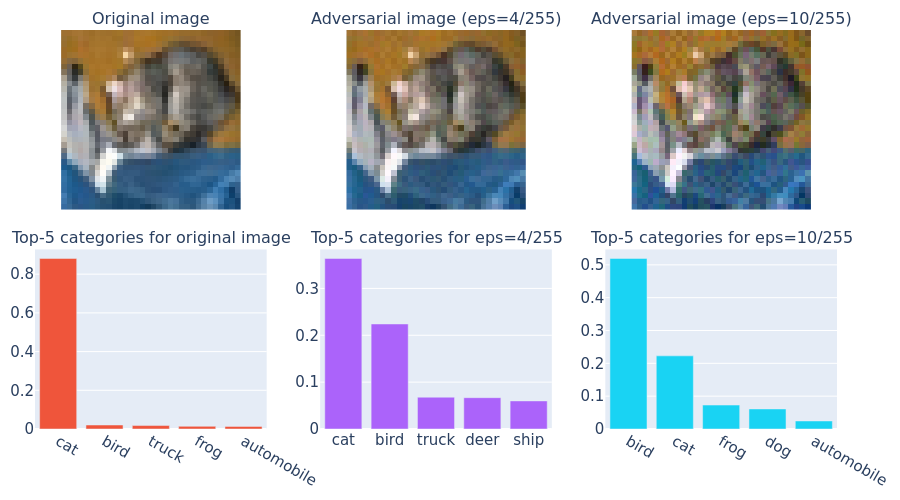
\includegraphics[width=0.9\textwidth]{images/fgsm_example_CIFAR10.png}
  \caption{Examples of the FGSM attack.}
  \label{fig:fgsm_examples_cifar10}
\end{figure}

\begin{figure}[H]
  \centering
  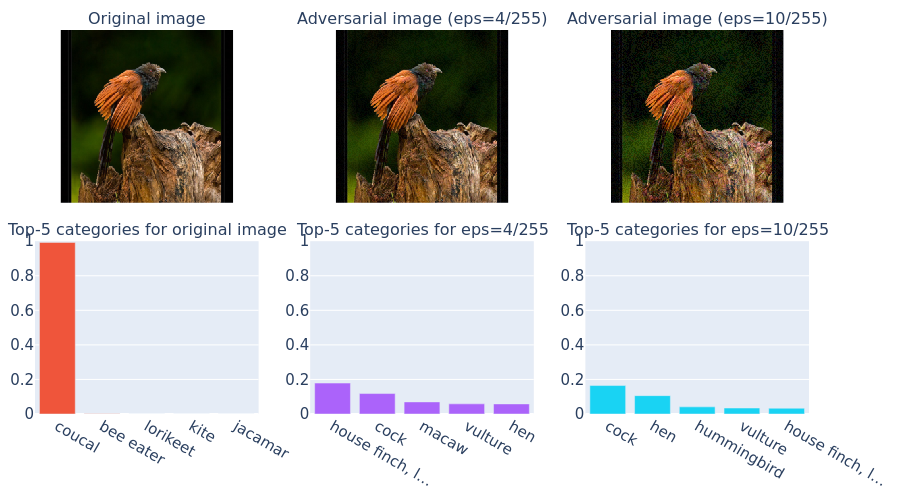
\includegraphics[width=0.9\textwidth]{images/fgsm_example_ImageNet.png}
  \caption{Examples of the FGSM attack.}
  \label{fig:fgsm_examples_imagenet}
\end{figure}

The attack seems to not work for the image from MNIST, but works well
on the one from CIFAR10 and ImageNet.
Is it the case for all images?

So I take the three classifiers, a thousand test images from each dataset,
compute the gradient of the loss with respect to the input image
and add $\e = 10 / 255$ times the sign of the gradient to the image.
This gives a thousand adversarial images for each task and
we can see the accuracy of the clean versus the adversarial images
in \autoref{fig:fgsm_eps10_agregate}.

\begin{figure}[H]
  \centering
  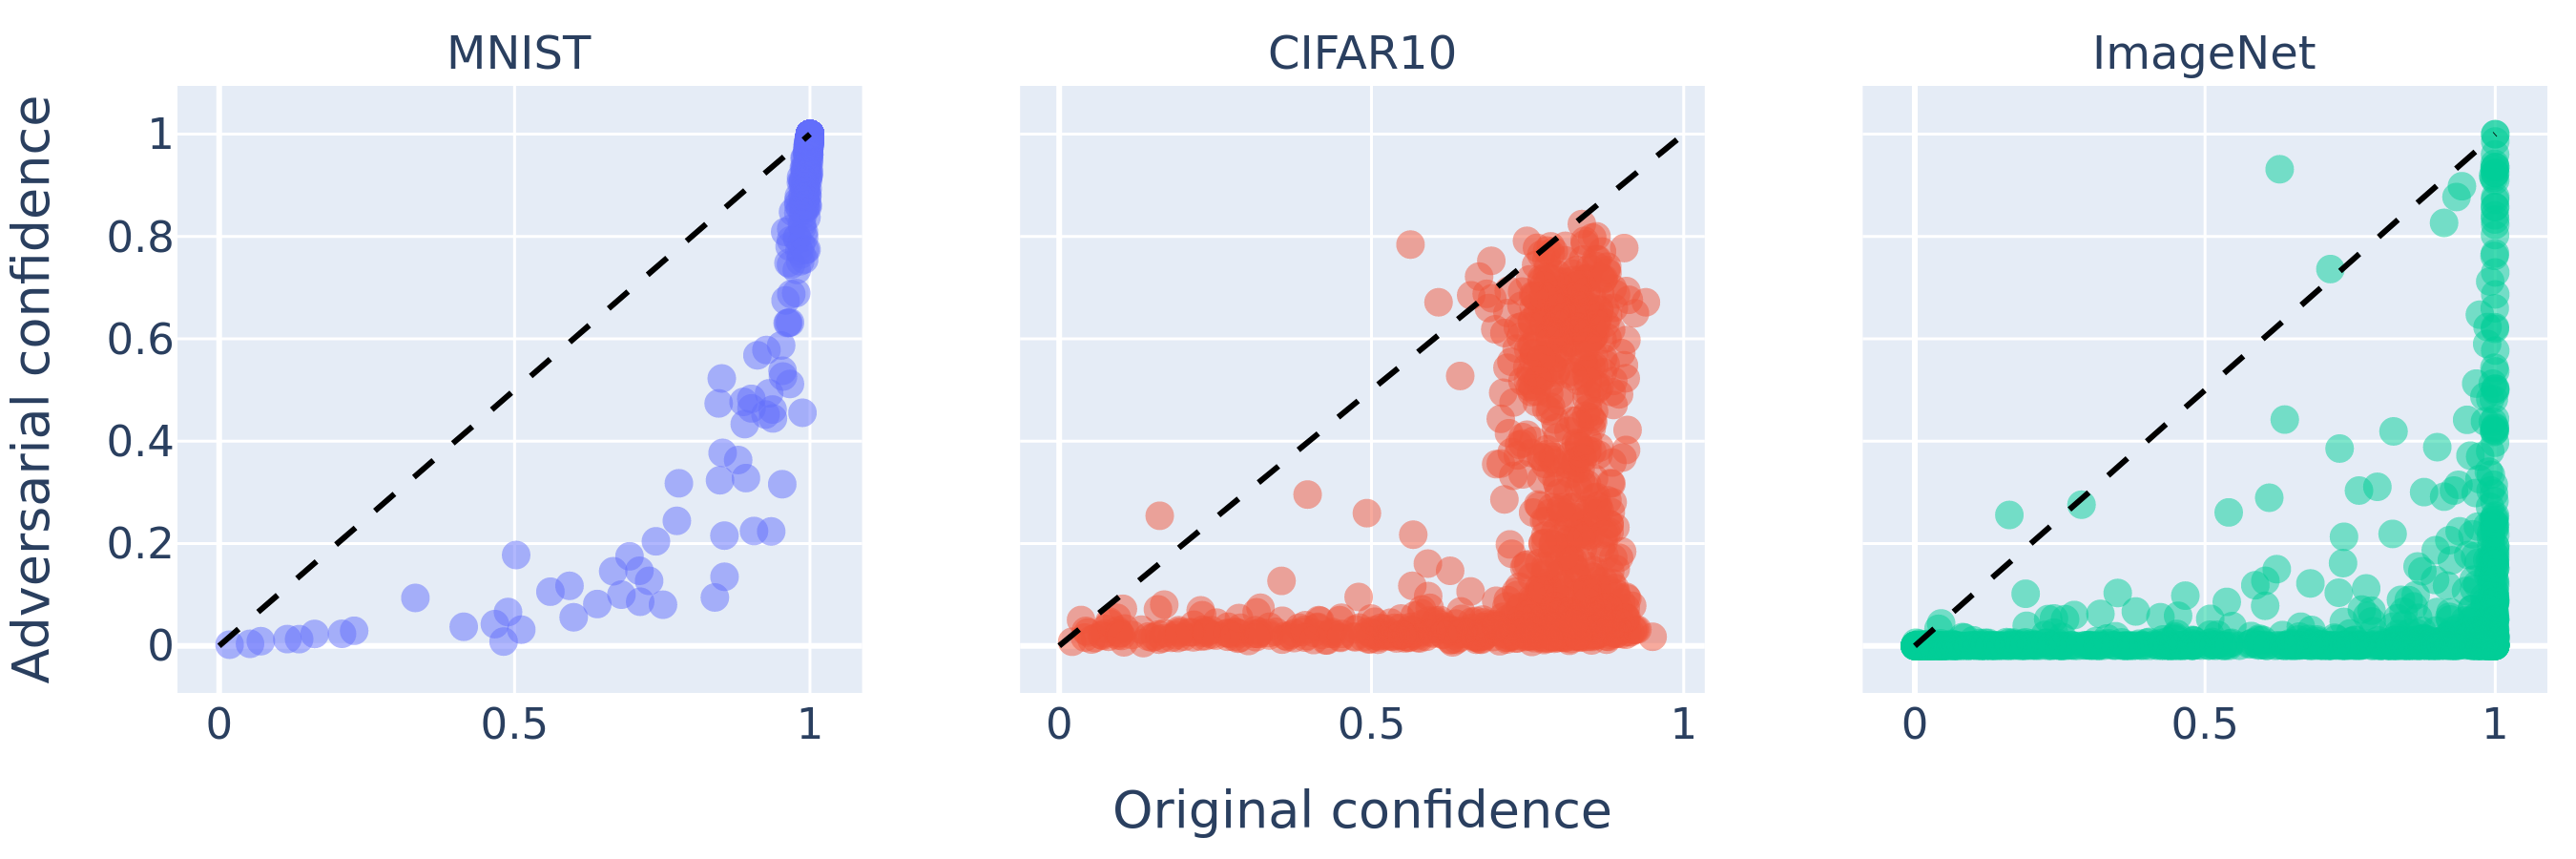
\includegraphics[width=0.9\textwidth]{images/fgsm_strength.png}
  \caption{Confidence of the three classifiers in the correct label of
    a 1000 test images before and after an FGSM attack with $\epsilon = 10 / 255$.
    The black line corresponds to no change in confidence.
  }
  \label{fig:fgsm_eps10_agregate}
\end{figure}

We can see that, on agregate, it works very well on ImageNet and CIFAR10,
and less well on MNIST. This can likely be attributed to the fact that
images from CIFAR10 and ImageNet are larger than MNIST and with three
color channels instead of one. The larger size allows for more ways to
find a path towards the decision boundary.
The sizes can be found in \autoref{fig:dataset_sizes}.

\begin{figure}[h]
  \centering
  \begin{tabular}{l|cccc}
    & MNIST & CIFAR10 & ImageNet \\ \hline
    Clean accuracy	& 98.9\,\%	& 92.8\,\%	& 77.2\,\%	& \\
    Accuracy $\epsilon=4/255$	& 98.8\,\%	& 87.2\,\%	& 50.2\,\%	& \\
    Accuracy $\epsilon=10/255$	& 98.8\,\%	& 76.8\,\%	& 28.2\,\%	& \\
    Image size & $1 \times 28 \times 28$ & $3 \times 32 \times 32$ & $3 \times 256 \times 256$\footnotemark
  \end{tabular}
  \caption{Top-1 accuracy before and after FGSM attack on a thousand images.}
  \label{fig:dataset_sizes}
\end{figure}

\footnotetext{
  ImageNet has images of different sizes, but were resized and croped
  to $256 \times 256$. This is different than the original paper
  \cite{He2015DeepRL} which used $224 \times 224$ images,
  but the classifier still acheives good accuracy.
  This design choice comes from the fact that the autoencoder
  used in the next section cannot take images smaller than $256 \times 256$.
}

\todo{Check that the footnote is on the same page as the figure}

\subsection{Iterated projected gradient descent}


\subsection{Universal and transferable attacks}

\subsection{Comparision}


\paragraph{Conclusion}

Competition \cite{Kurakin2018AdversarialAA}









\newpage

\section{Attacking autoencoders}

Autoencoders have been suggested as a defense mechanism against adversarial attacks
\cite{guo2017countering,liu2017enhanced,liu2018feature}.

\subsection{Autoencoders}

Autoencoders where introduced by \cite{hinton2006reducing} as a way to learn
a low dimensional representation of data.
They are a class of neural networks that are trained to reconstruct their input,
and are composed of two deep neural network, an encoder and a decoder with a bottleneck in between
as shown in \autoref{fig:autoencoder}.

\begin{figure}[h]
  \centering
  \begin{tikzpicture}
    % Encoder, a trapeze
    \draw[atomictangerine, fill=atomictangerine!20]
      (0, 0) -- (0, 4) -- (4, 3) -- (4, 1) -- cycle;
    \node[] at (2, 2) {Encoder};
    % Bottleneck, vertical text, no shape
    \node[rotate=-90] at (4.5, 2) {Bottleneck};
    % Decoder, a trapeze
    \draw[airforceblue, fill=airforceblue!20]
      (5, 1) -- (5, 3) -- (9, 4) -- (9, 0) -- cycle;
    \node[] at (7, 2) {Decoder};

    % Text input on the left, vertical
    \node[rotate=-90] at (-1, 2) {Input}
      edge[->, thick] (-0, 2);
    % Text output on the right, vertical
    \node[rotate=-90] at (10, 2) {Output}
      edge[<-, thick] (9, 2);
  \end{tikzpicture}
  \caption{Overview of the autoencoder architecture}
  \label{fig:autoencoder}
\end{figure}

The \emph{encoder} takes an high dimensional data point as input,
processes it through a series of layers, usually fully connected layers
or a residual network \cite{He2015DeepRL} in the case of visual data,
and outputs a low dimensional representation of the input.

The \emph{decoder} takes the low dimensional output of the encoder and
processes it similarly through a series of layers,
and outputs a high dimensional reconstruction of the input.

The \emph{bottleneck} is not a layer, but rather the middle of the autoencoder,
where the activations are the lowest number of dimensions.

\paragraph{Training}
Autoencoders are trained to reconstruct their input,
that is, they learn the identity function. The loss is a natural metric
on the data space, such as the mean squared error for real valued data.

\begin{definition}
  The \emph{reconstruction loss} for an autoencoder $f$ on an input $x \in \Xx$
  is
  \[
    \Ll_{\text{recon.}}(x) = \norm{x - f(x)}^2
  \]
\end{definition}

To prevent overfitting and to perform a directly useful task,
an autoencoder can be train to reconstruct a noisy or corrupted
version of the input.
\begin{definition}
  The \emph{denoising loss} for an autoencoder $f$ on an input $x \in \Xx$ is
  \[
    \Ll_{\text{denoising}}(x) = \norm{x - f(x + \e)}^2
  \]
  where \e is a random vector of the same dimension as $x$, of white noise
  whose variance is an hyperparmeter of the training setup.

  Note that the denoising loss is stochastic, as it depends on the random
  vector \e. In practice, we use the compute the loss on one sample of \e
  per input.
\end{definition}

\paragraph{Variational autoencoders}
An specific kind of autoencoders intruduced by \todo{ref intro VAE}
are variational autoencoders (VAE).
Technically, they are not very different from regular autoencoders,
but they come from a different background than data compression.
Indeed, the hope is that VAEs model the process from which the data was generated.
Oftentimes, we expect a datapoint (for instance the image of a leaf) to be determined
only by \textit{a few} variables (for instance, the species of the tree, its age,
the season, the angle at which the picture was taken etc.).
We will call $P$, the vector of those few variables that generate the datapoint.

The encoder of a VAE tries to find some representation of $P$ and outputs two vectors,
$\mu$ and $\sigma$ instead of one, which are interpreted as the mean and the variance
of the prior on $P$, which is assumed to be a normal distribution.

The variable $P \sim \Nn(\mu, \sigma)$ are then sampled
and fed to the decoder that tried to reconstruct what should be
generated from the underlying variables. The decoder thus tries
to model the process that generated the dataset and outputs
a distribution $Q$ over the data space.

\begin{definition}
  Let $f$ be a VAE and $x \in \Xx$ a datapoint.
  It loss on $x$ is composed of two terms,
  the \emph{likelyhood loss} and the \emph{regularisation loss}.
  \[
    \Ll_{\text{vae}}(x) =
      \underbrace{\IP(x \mid f(x))}
        _{\text{likelyhood loss}}
      + \underbrace{\KLdiv{P}{\Nn(0, 1)}}
        _{\text{regularisation loss}}
  \]

\end{definition}

\begin{remark}
  The KL divergence is a measure of how different two distributions are.
  In this case, it is used to measure how far the prior on $P$ is from
  the standard normal distribution.
  \[
    \KLdiv{P}{Q} = \int_{\Xx} P(x) \log \frac{P(x)}{Q(x)} \,\dd x
  \]

  Here we can use the fact that both $P$ and $Q$ are $n$-dimensional normal distributions
  to compute the KL divergence in closed form.
  \[
    \KLdiv{\Nn(\mu, \sigma)}{\Nn(0, 1)}
    = \frac{-1}{2n} \sum_{i=1}^{n} \Par{
      1 + \log \sigma_i^2 - \mu_i^2 - \sigma_i^2
    }
  \]
\end{remark}

\todo{Say why KL is used}

\paragraph{$\beta$-VAE}

\subsection{Attacks}
Autoencoders can be used to prevent adversarial attacks
against classifier by prepocessing images through the autoencoder.
The setup is shown in \autoref{fig:ae_defense}.

\begin{figure}[h]
  \centering

  \begin{tikzpicture}[scale=0.8]
    \begin{scope}[local bounding box=autoencoder]
      % Encoder
      \draw[atomictangerine, fill=atomictangerine!20]
        (0, 0) -- (0, 4) -- (4, 3) -- (4, 1) -- cycle;
      \node[] at (2, 2) {Encoder};
      % Decoder
      \draw[airforceblue, fill=airforceblue!20]
        (5, 1) -- (5, 3) -- (9, 4) -- (9, 0) -- cycle;
      \node[] at (7, 2) {Decoder};
      \path[->, thick] (4, 2) --
       node[rotate=-90] {Bottleneck}
       (5, 2);
      % \node[rotate=-90, red] (bottleneck) at (4.5, 2) {Bottleneck};
    \end{scope}

    % Box around the autoencoder, spacing of 0.5 around
    \draw[thick, rounded corners=0cm]
      ($(autoencoder.north west) + (-0.5, 0.5)$) rectangle
      ($(autoencoder.south east) + (0.5, -0.5)$);
    % Label for the autoencoder
    \node[anchor=south] at ($(autoencoder.north) + (0, 0.5)$) {Autoencoder};

    % Text input on the left, vertical
    \node[rotate=-90] at (-1, 2) {Input}
      edge[->, thick] (autoencoder.west);

    % Classifier
    \begin{scope}[local bounding box=classifier]
      \draw[awesome!80, fill=awesome!20] (autoencoder.south east)
        ++(1, 0) -- ++(0, 4) -- ++(4, -1) -- ++(0, -2) -- cycle;
      \node[] at (12, 2) {Classifier};
    \end{scope}

    % Arrow from the autoencoder to the classifier
    \draw[->, thick] (autoencoder.east) -- ++(1, 0);

    % Text output on the right, vertical
    \node[rotate=-90] at ($(classifier.east) + (1, 0)$) {Classification}
      edge[<-, thick] (classifier.east);

  \end{tikzpicture}

  \caption{Autoencoder used as a defense against adversarial attacks}
  \label{fig:ae_defense}
\end{figure}

The hope is that an adversarial perturbation of the input
will not pass through the bottleneck of the autoencoder,
and thus will not be able to fool the classifier.
Indeed, the bottleneck is small, and therefore information
constrained, so we expect to the autoencoder to
not faithfully reconstruct patterns that it has never seen
during training. In particular, we expect the latent respresentation
of an adversarial input to be the same as the representation of
the original input, and thus the autoencoder should reconstruct the
original input when fed the adversarial one.

\paragraph{} We can verify this empirically.

% Vary:
% - autoencoder/task
% - pairs of inputs
% Histogram with:
% - line 1: distance between latent representation of original and adversarial
% - line 2: distance between random pairs
% - line 3: distance between random pairs of the same class

\section{Phase transition: ease of attack}

\section{Phase transition: norm detection}


\section*{Conclusion}
\addcontentsline{toc}{section}{Conclusion}

...

\newpage
\nocite{*}
\addcontentsline{toc}{section}{References}
\bibliographystyle{apalike}
\bibliography{bibliography.bib}

\end{document}
